\documentclass[aspectratio=169]{beamer}
\usepackage[deluxe]{luatexja-preset}
\renewcommand{\kanjifamilydefault}{\gtdefault}
\usepackage{minted}
\usepackage{xcolor}
\usepackage{hyperref}
\usepackage{amsmath}
\setbeamertemplate{navigation symbols}{}

\title{テスト駆動開発 ハンズオン \#1}
\subtitle{Test-Driven Development Hans-On \#1}
\author{asuka y}
\date{Aug 21 2022}

\begin{document}

\begin{frame}
  \titlepage
\end{frame}

\section*{INDEX}
\begin{frame}
  \frametitle{テスト駆動揮発ハンズオン \#1}
  \tableofcontents
\end{frame}

\section{テスト駆動開発とは何か}
\subsection{テスト駆動開発とは何か}
\begin{frame}\frametitle{テスト開発とは何か}
  \begin{quote}
    テスト駆動開発(TDD)はテスト技法ではない...
    TDDは分析器用であり、設計技法であり、
    実際には開発のすべてのアクティビティを構造化する技法なのだ。
  \end{quote}
  \begin{flushright}
    ---Kent Beck
  \end{flushright}

  テスト技法ではなく、開発技法である。

  {
    \large \color{blue}
    $\rightarrow$
    テストを書くことが目的ではない。
  }
\end{frame}

\subsection{テスト駆動開発が目指すもの}
\begin{frame}\frametitle{テスト駆動開発が目指すもの}
  \begin{quote}
    「動作するきれいなコード」。
    Ron Jeffiresのこの簡潔な言葉が、
    テスト駆動開発(TDD)のゴールだ。
    動作するきれいなコードはあらゆる意味で価値がある。
  \end{quote}
  \begin{flushright}
    ---Kent Beck
  \end{flushright}

  TDDは動作する「きれいなコード」に辿り着くために、
  {\color{blue} 自動化されたテストによって開発を推し進める技法}である。

  \begin{center}
    \color{red} \large テストを手段として用いるのであって、テストが目的なのではない。
  \end{center}
\end{frame}

\begin{frame}[fragile]\frametitle{動作するきれいなコード}
  \begin{itemize}
    \item 開発が予測可能になる。何が完成していて、何が完成していないかがわかる。
    \item コードが伝えようとしていることを余すところなく受け取れる。
      最初に思いついたコードを書き殴っただけで終わりなら、
      最高してより良いコードを書くチャンスは永遠に来ない。

    \large \color{blue}
    \item あなたが作るソフトウェアのユーザを快適にする。
    \item チームメイトはあなたを信頼し、あなたもまたチームメイトを信頼する。
    \item 書いていて気持ちがいい。
  \end{itemize}
\end{frame}

\subsection{テスト駆動開発の進め方}
\begin{frame}\frametitle{テスト駆動開発の進め方}
  \begin{enumerate}
    \item まずはテストを1つ書く
    \item すべてのテストを走らせ、新しいテストの失敗を確認する
    \item 小さな変更を行う
    \item すべてのテストを走らせ、すべて成功することを確認する
    \item リファクタリングを行って重複を排除する
  \end{enumerate}

  \begin{center}
    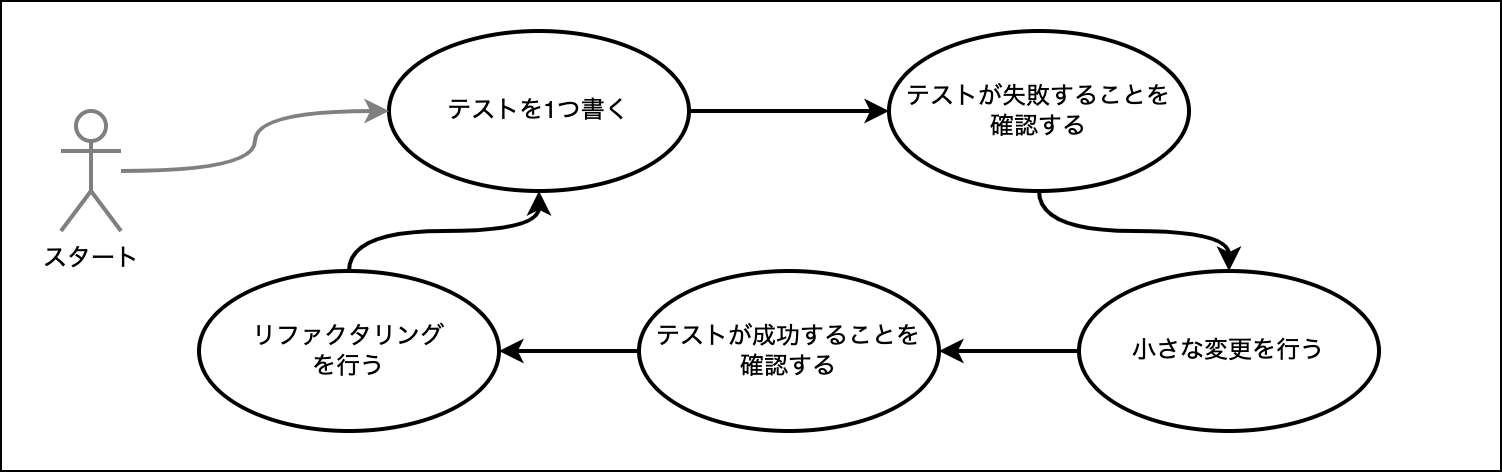
\includegraphics[height=4cm]{asset/tdd_cycle.png}
  \end{center}
\end{frame}

\begin{frame}[fragile]\frametitle{まずはテストを1つ書く}
  これから何を開発しないといけないのか、をはじめに考える。

  \begin{quote}
    \color{blue}
    2つの整数の和を知りたい。
  \end{quote}
  $\rightarrow$ 2つの引数を取って、和を返す関数を作れば良いんだな。

  \scriptsize
  \begin{minted}{go}
    /*-- lib.go --*/
    func Add(a, b int) int {
        return 0
    }

    /*-- lib_test.go --*/
    func TestAdd(t *testing.T) {
        result := Add(3, 4)
        if result != 7 {
            t.Fatalf("want=%d, got=%d", 7, result)
        }
    }
  \end{minted}
\end{frame}

\begin{frame}[fragile]\frametitle{全てのテストを走らせ、新しいテストの失敗を確認する}
  \scriptsize
  \begin{minted}{text}
    example % go test -cover .
    --- FAIL: TestAdd (0.00s)
        lib_test.go:10: want=7, got=0
    FAIL
    coverage: 100.0% of statements
    FAIL	github.com/a-skua/tdd-handson/example	0.199s
    FAIL
  \end{minted}
\end{frame}

\begin{frame}[fragile]\frametitle{小さな変更を行う}
  \scriptsize
  \begin{minted}{go}
    /*-- lib.go --*/
    func Add(a, b int) int {
        return a + b
    }
  \end{minted}
\end{frame}

\begin{frame}[fragile]\frametitle{全てのテストを走らせ、全て成功することを確認する}
  \scriptsize
  \begin{minted}{text}
    example % go test -cover .
    ok  	github.com/a-skua/tdd-handson/example	0.226s	coverage: 100.0% of statements
  \end{minted}
\end{frame}

\begin{frame}[fragile]\frametitle{リファクタリングを行なって重複を排除する}
  これで1サイクルが終了する。
  \scriptsize
  \begin{minted}{go}
    /*-- lib.go --*/
    func Add(a, b int) int {
        return a + b
    }

    /*-- lib_test.go --*/
    func TestAdd(t *testing.T) {
        result := Add(3, 4)
        if result != 7 {
            t.Fatalf("want=%d, got=%d", 7, result)
        }
    }
  \end{minted}
\end{frame}

\begin{frame}[fragile]\frametitle{まずはテストを1つ書く}
  2サイクル目に入る

  \begin{quote}
    \color{blue}
    3つの整数の和を知りたい。
  \end{quote}
  $\rightarrow$ 3つの引数を取って、和を返す関数を作れば良いんだな。

  \scriptsize
  \begin{minted}{go}
    /*-- lib.go --*/
    func Add3(a, b, c int) int {
        return 0
    }

    /*-- lib_test.go --*/
    func TestAdd3(t *testing.T) {
        result := Add(3, 4, 5)
        if result != 12 {
            t.Fatalf("want=%d, got=%d", 12, result)
        }
    }
  \end{minted}
\end{frame}

\begin{frame}[fragile]\frametitle{全てのテストを走らせ、新しいテストの失敗を確認する}
  \scriptsize
  \begin{minted}{text}
    example % go test -cover .
    --- FAIL: TestAdd3 (0.00s)
        lib_test.go:17: want=12, got=0
    FAIL
    coverage: 100.0% of statements
    FAIL	github.com/a-skua/tdd-handson/example	0.233s
    FAIL
  \end{minted}
\end{frame}

\begin{frame}[fragile]\frametitle{小さな変更を行う}
  \scriptsize
  \begin{minted}{go}
    /*-- lib.go --*/
    func Add3(a, b, c int) int {
        return a + b + c
    }
  \end{minted}
\end{frame}

\begin{frame}[fragile]\frametitle{全てのテストを走らせ、全て成功することを確認する}
  \scriptsize
  \begin{minted}{text}
    example % go test -cover .
    ok  	github.com/a-skua/tdd-handson/example	0.226s	coverage: 100.0% of statements
  \end{minted}
\end{frame}

\begin{frame}[fragile]\frametitle{リファクタリングを行なって重複を排除する}
  2サイクル目の終了
  \scriptsize
  \begin{minted}{go}
    /*-- lib.go --*/
    package example

    func Add(a, b int) int {
        return sum(a, b)
    }

    func Add3(a, b, c int) int {
        return sum(a, b, c)
    }

    func sum(ns ...int) (result int) {
        for _, n := range ns {
            result += n
        }
        return
    }
  \end{minted}
  ---
  \begin{minted}{text}
    example % go test -cover .
    ok  	github.com/a-skua/tdd-handson/example	0.213s	coverage: 100.0% of statements
  \end{minted}
\end{frame}

\section{ハンズオン}
\subsection{フィボナッチ数列}
\begin{frame}\frametitle{ハンズオン: フィボナッチ数列}
\end{frame}

\subsection{逆ポーランド電卓}
\begin{frame}\frametitle{ハンズオン: 逆ポーランド電卓}
\end{frame}

\subsection{RESTful API}
\begin{frame}\frametitle{ハンズオン: RESTful API}
\end{frame}

\end{document}
